\documentclass{standalone}
\usepackage{circuitikz}
\usepackage{schemabloc}

\begin{document}
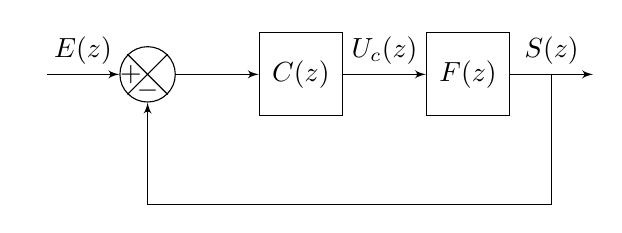
\begin{tikzpicture}
\sbEntree{E}
\sbComp{comp}{E}
\sbRelier[$E(z)$]{E}{comp}
\sbBloc[3]{B1}{$C(z)$}{comp}
\sbRelier{comp}{B1}
\sbBloc[3]{B2}{$F(z)$}{B1}
\sbRelier[$U_c(z)$]{B1}{B2}
\sbSortie[3]{S}{B2}
\sbRelier[$S(z)$]{B2}{S}
\sbRenvoi{B2-S}{comp}{}
\end{tikzpicture}
\end{document}